% !TeX root = enterprise-architecture-digital-blueprint.tex
% !TeX encoding = UTF-8
\chapter{Business Case dan Portofolio Inisiatif}
\label{ch:ch13-business-case}

% Gaya listing Python khusus bab ini. Preamble modul tidak memuat gaya Python.
\lstdefinestyle{ch13python}{
  language=Python,
  basicstyle=\ttfamily\scriptsize,
  keywordstyle=\color{blue}\bfseries,
  commentstyle=\color{gray}\itshape,
  stringstyle=\color{red},
  numbers=left,
  numberstyle=\tiny\color{gray},
  breaklines=true,
  frame=lines,
  backgroundcolor=\color{lightgray!10},
  tabsize=2,
  showstringspaces=false,
  captionpos=b
}

\section*{Tujuan Pembelajaran}
\begin{itemize}
  \item Menyusun \textit{business case} untuk inisiatif prioritas dengan manfaat, biaya, risiko, dan asumsi yang eksplisit.
  \item Memetakan manfaat ke perubahan bisnis dan pemungkinnya dengan \textit{benefits dependency network}.
  \item Memprioritaskan portofolio inisiatif dengan kriteria berbobot dan menjustifikasi hasilnya.
\end{itemize}

\section{Pendahuluan}

Banyak proyek Teknologi Informasi (TI) disetujui dengan alasan yang terdengar
meyakinkan: sistem lama sudah usang, vendor menawarkan fitur baru, atau unit
lain sudah memakainya. Proyeknya berjalan, sistemnya terpasang, dan laporan
penutupan menyatakan proyek selesai tepat waktu dan sesuai anggaran. Setahun
kemudian seorang komisaris bertanya, ``Apa hasil investasi itu bagi
organisasi?'' Tidak ada yang dapat menjawab. Sejak awal tidak ada yang
menetapkan hasil apa yang diharapkan, siapa yang bertanggung jawab
mewujudkannya, dan bagaimana mengukurnya.

Bab 12 menghasilkan peta jalan 2026 sampai 2030, yaitu urutan arsitektur
transisi dan paket kerja. Peta jalan menjawab pertanyaan ``apa yang dikerjakan
lebih dahulu''. Sebelum menyetujui anggaran, direksi masih punya dua
pertanyaan lain. Pertama, mengapa sebuah inisiatif layak didanai. Kedua,
inisiatif mana yang didanai bila uangnya tidak cukup untuk semua. Bab ini
menjawab pertanyaan pertama lewat \textit{business case} untuk satu inisiatif,
dan pertanyaan kedua lewat prioritas untuk seluruh portofolio inisiatif.
Keduanya mengubah cetak biru dari dokumen rancangan menjadi rencana yang dapat
didanai.

Rujukan utama bab ini adalah pendekatan manajemen manfaat dari Ward dan Daniel
\cite{ward2012}, beserta \textit{benefits dependency network} yang dirumuskan
Peppard, Ward, dan Daniel \cite{c13-peppard2007}. Teknik penilaian nilai bisnis
pada perencanaan migrasi diambil dari The Open Group Architecture Framework
(TOGAF) \cite{togaf10}, sedangkan struktur \textit{business case} mengikuti
panduan HM Treasury \cite{c13-hmt2026}. Temuan Flyvbjerg dan Budzier tentang
pembengkakan biaya proyek TI \cite{flyvbjerg2011} dipakai untuk menjaga
agar angka di dalam \textit{business case} tetap jujur.

\IfFileExists{../figures/ch13-diagram-konsep.png}{%

Gambar \ref{fig:ch13-ilustrasi-bab} merangkum hubungan komponen dan konsep utama bab ini.
\begin{figure}[!htb]
  \centering
  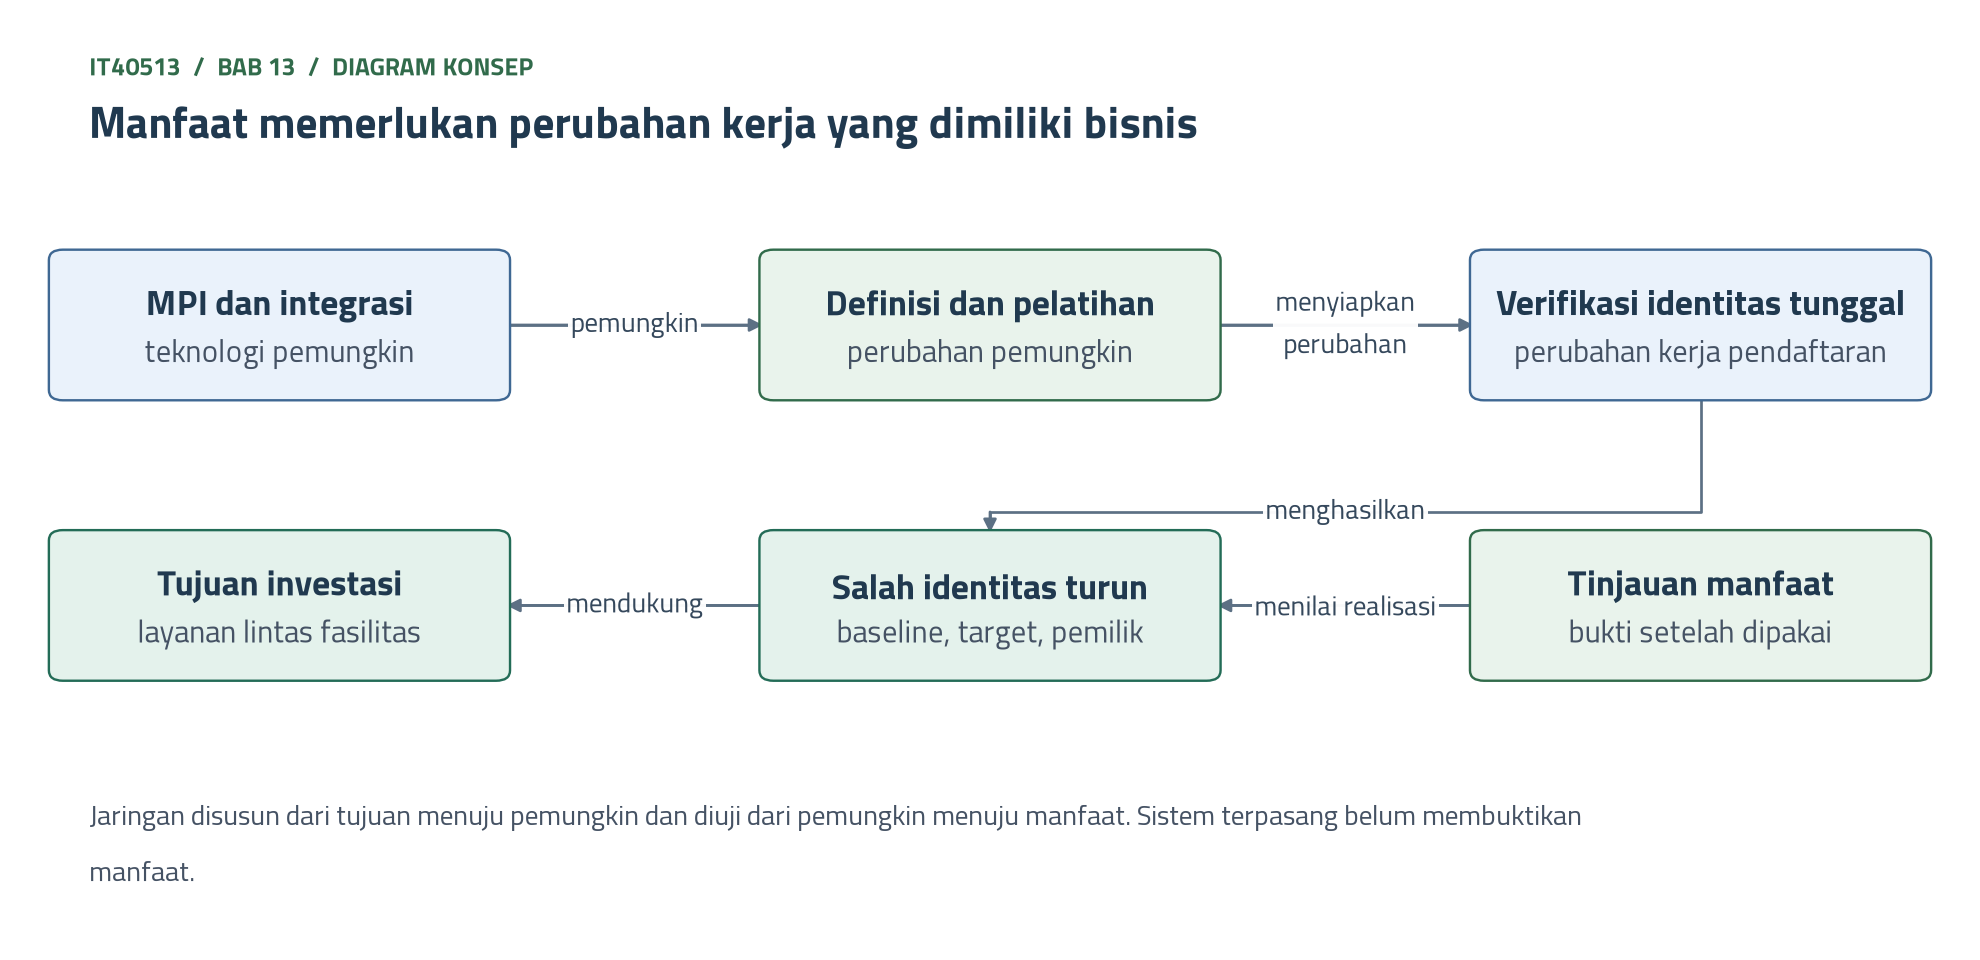
\includegraphics[width=\textwidth]{../figures/ch13-diagram-konsep.png}
  \caption{Manfaat memerlukan perubahan kerja yang dimiliki bisnis}
  \label{fig:ch13-ilustrasi-bab}
\end{figure}
}{}

\section{Manajemen Manfaat}

Manajemen manfaat (\textit{benefits management}) adalah proses mengatur sebuah
investasi TI agar manfaat yang dijanjikan benar-benar terwujud, bukan hanya
agar sistemnya terpasang \cite{ward2012}. Gagasan dasarnya sederhana.
Teknologi sendiri tidak menghasilkan manfaat. Manfaat muncul ketika orang
bekerja dengan cara baru yang dimungkinkan oleh teknologi itu. Karena itu
manfaat dinyatakan sebagai perubahan pada ukuran kinerja yang dirasakan pihak
tertentu, misalnya waktu tunggu pasien atau nilai klaim yang tertunda, bukan
sebagai daftar kemampuan sistem.

Analoginya seperti membeli \textit{treadmill}. Alat itu punya fitur: kecepatan
yang dapat diatur, pengukur detak jantung, dan program latihan. Tidak satu pun
fitur itu menurunkan berat badan. Berat badan turun bila pemiliknya berlatih
tiga kali seminggu dan mengubah pola makan. \textit{Treadmill} yang dibeli
tanpa perubahan kebiasaan berakhir menjadi gantungan baju, padahal ``proyek
pembelian''-nya selesai tepat waktu dan sesuai anggaran.

Tabel \ref{tab:ch13-fitur-manfaat} memperlihatkan perbedaan fitur dan manfaat
pada empat contoh dari Medikara Health. Contoh pertama memakai Master Patient
Index (MPI), yaitu indeks identitas pasien tunggal yang dirancang di Bab 9.
Kolom paling kanan berisi perubahan cara kerja yang harus terjadi agar fitur
berubah menjadi manfaat.

\begin{table}[!htb]
  \centering
  \caption{Fitur, manfaat, dan perubahan cara kerja pada empat contoh Medikara}
  \label{tab:ch13-fitur-manfaat}
  \footnotesize
  \begin{tabularx}{\textwidth}{>{\raggedright\arraybackslash}X
                               >{\raggedright\arraybackslash}X
                               >{\raggedright\arraybackslash}X}
    \hline
    \textbf{Fitur yang dibeli} & \textbf{Manfaat yang diharapkan} &
      \textbf{Perubahan cara kerja yang dibutuhkan} \\
    \hline
    Pencarian pasien di MPI & Pendaftaran pasien lama turun dari 6 menjadi
      3 menit & Petugas mencari pasien lebih dahulu sebelum membuat rekam
      medis baru \\
    \hline
    Janji temu daring di Medikara+ & Antrean loket pagi berkurang & Dokter
      membuka kuota jadwal di aplikasi, bukan hanya di loket \\
    \hline
    \textit{Dashboard} laporan terpadu & Rapat bulanan tanpa rekonsiliasi angka
      & Unit berhenti menyusun \textit{spreadsheet} sendiri \\
    \hline
    Peninjauan hak akses otomatis & Temuan audit kontrol akses ditutup &
      Atasan meninjau hak akses bawahannya tiap triwulan \\
    \hline
  \end{tabularx}
\end{table}

Pembedaan ini punya dua konsekuensi. Pertama, perubahan cara kerja harus
direncanakan, dianggarkan, dan dipantau seperti perangkat lunaknya. Pelatihan,
aturan baru, dan pengalihan tugas petugas punya biaya dan jadwal. Kedua,
setiap manfaat butuh pemilik dari sisi bisnis. Pemilik manfaat (\textit{benefit
owner}) adalah orang yang menerima manfaat itu dan punya wewenang untuk
mengubah cara kerja unitnya \cite{ward2012}. Manajer proyek TI tidak cocok
menjadi pemilik manfaat. Tugasnya selesai ketika sistem diserahkan, sedangkan
manfaat baru terlihat berbulan-bulan sesudahnya.

Pertanyaan kemudian muncul: kapan manfaat dikelola? Ward dan Daniel
menyusunnya sebagai siklus lima tahap \cite{ward2012}, seperti pada Gambar
\ref{fig:ch13-siklus}. \textit{Business case} disusun pada tahap pertama dan
kedua. Tahap ketiga berjalan bersama proyek. Tahap keempat adalah tinjauan
sesudah sistem dipakai, ketika pemilik manfaat melaporkan apakah targetnya
tercapai. Tahap kelima mencari manfaat tambahan yang baru terlihat setelah
cara kerja berubah, lalu membawanya ke investasi berikutnya.

\begin{figure}[!htb]
  \centering
  \begin{tikzpicture}[
  font=\scriptsize,
  tahap/.style={draw, rounded corners, minimum height=1.25cm, text width=1.85cm,
                align=center, font=\scriptsize\bfseries},
  panah/.style={-{Stealth[length=2mm]}, thick}
]
  \node[tahap, fill=blue!8] (t1) at (0,0)
    {{\tiny\mdseries Tahap 1}\\Identifikasi dan susun manfaat};
  \node[tahap, fill=blue!8] (t2) at (2.45,0)
    {{\tiny\mdseries Tahap 2}\\Rencanakan realisasi manfaat};
  \node[tahap, fill=blue!8] (t3) at (4.9,0)
    {{\tiny\mdseries Tahap 3}\\Jalankan rencana manfaat};
  \node[tahap, fill=orange!12] (t4) at (7.35,0)
    {{\tiny\mdseries Tahap 4}\\Tinjau dan evaluasi hasil};
  \node[tahap, fill=green!10] (t5) at (9.8,0)
    {{\tiny\mdseries Tahap 5}\\Temukan manfaat lanjutan};

  \draw[panah] (t1) -- (t2);
  \draw[panah] (t2) -- (t3);
  \draw[panah] (t3) -- (t4);
  \draw[panah] (t4) -- (t5);
  \draw[panah] (t5.south) -- ++(0,-0.6) -| (t1.south);
  \node[font=\tiny, gray, fill=white, inner sep=1pt] at (4.9,-1.23)
    {investasi berikutnya memakai pelajaran dari siklus ini};

  \draw[gray, thick] ([yshift=0.15cm]t1.north west) -- ++(0,0.15)
    -- ([yshift=0.3cm]t2.north east) -- ++(0,-0.15);
  \node[font=\tiny, anchor=south] at ($(t1.north)!0.5!(t2.north)+(0,0.32)$)
    {\textit{business case} disusun di sini};
  \node[font=\tiny, anchor=south] at ([yshift=0.15cm]t3.north)
    {proyek berjalan};
  \node[font=\tiny, anchor=south] at ([yshift=0.15cm]t4.north)
    {pemilik manfaat melapor};
\end{tikzpicture}

  \caption{Siklus manajemen manfaat lima tahap menurut Ward dan Daniel. Tahap
           keempat ditandai karena tahap itulah yang membuktikan apakah
           investasinya berhasil}
  \label{fig:ch13-siklus}
\end{figure}

Tahap keempat menyambung langsung ke tata kelola arsitektur di Bab 14. Tanpa
forum yang meminta laporan realisasi manfaat, tahap ini mudah dilewati, dan
siklusnya berhenti di tahap ketiga. Organisasi lalu kembali ke keadaan di
awal bab: proyek selesai, tetapi tidak ada yang tahu hasilnya.

\subsection*{Manfaat yang dapat dicairkan dan yang tidak}

Dua hal pada manfaat sering tertukar. Pembagiannya begini. Manfaat yang dapat
dicairkan (\textit{cashable}) mengubah angka di laporan keuangan, yaitu biaya
yang benar-benar hilang atau pendapatan yang benar-benar bertambah. Manfaat
yang tidak dapat dicairkan tetap nyata, tetapi tidak mengubah angka keuangan
kecuali ada keputusan tambahan. Dua contoh:

\begin{enumerate}
  \item Misalkan MPI memangkas waktu pendaftaran pasien lama dari 6 menit
        menjadi 3 menit. Sekitar 70 persen dari 1,2 juta kunjungan per tahun
        adalah pasien lama, yaitu 840.000 kunjungan. Waktu yang dihemat
        mencapai 2.520.000 menit atau 42.000 jam kerja petugas. Angka itu
        tidak mengurangi gaji siapa pun. Penghematan baru menjadi uang bila
        Medikara memutuskan, misalnya, tidak menambah petugas pendaftaran
        ketika membuka klinik baru.
  \item Penghentian rekonsiliasi laporan manual membebaskan sekitar 640 jam
        kerja analis per bulan, setara empat orang analis. Manfaat ini
        bernilai Rp400 juta per tahun hanya bila keempat analis itu dialihkan
        ke pekerjaan yang selama ini dikerjakan tenaga kontrak, sehingga
        biaya kontrak itu benar-benar hilang.
\end{enumerate}

Pembedaan ini menentukan isi \textit{business case}. Manfaat yang dapat
dicairkan masuk ke perhitungan finansial. Manfaat yang tidak dapat dicairkan
tetap ditulis, lengkap dengan ukurannya, tetapi tidak dijumlahkan sebagai
rupiah. Menjumlahkan 42.000 jam sebagai uang membuat angka terlihat besar,
dan direktur keuangan yang teliti akan mencoretnya.

\section{Benefits Dependency Network}

\textit{Benefits dependency network} adalah diagram sebab akibat yang
menghubungkan tujuan investasi dengan teknologi yang memungkinkannya, lewat
manfaat dan perubahan yang dibutuhkan di antara keduanya \cite{ward2012}.
Jaringan ini punya lima kolom. Dari kanan ke kiri: tujuan investasi, manfaat
bisnis, perubahan bisnis, perubahan pemungkin, dan teknologi pemungkin.
Peppard, Ward, dan Daniel meringkas ketiga lapisannya sebagai tujuan akhir
(\textit{ends}), cara kerja baru (\textit{ways}), dan sarana teknologi
(\textit{means}). Jaringan itu juga mencatat siapa yang bertanggung jawab atas
tiap perubahan dan tiap manfaat \cite{c13-peppard2007}.

Jaringan ini dibaca dari dua arah. Penyusunannya dimulai dari kanan. Tim
bertanya: manfaat apa yang dibutuhkan untuk mencapai tujuan ini? Perubahan
cara kerja apa yang menghasilkan manfaat itu? Apa yang harus disiapkan agar
perubahan itu terjadi? Teknologi apa yang dibutuhkan? Teknologi dipilih paling
akhir, sesudah jelas untuk apa teknologi itu dibutuhkan. Pemeriksaannya
berjalan dari kiri. Tim bertanya: bila teknologi ini tersedia dan perubahan
ini dijalankan, apakah manfaat itu benar-benar muncul? Mata rantai yang tidak
lolos pemeriksaan ini adalah titik tempat manfaat akan hilang.

Analoginya seperti rencana menaikkan panen sebuah desa. Tujuannya pendapatan
petani naik. Manfaat yang dibutuhkan adalah gabah per petak bertambah.
Manfaat itu datang dari perubahan cara bertani: jadwal tanam serempak dan
pemupukan yang tepat waktu. Perubahan itu baru mungkin bila kelompok tani
menyepakati aturan pembagian air dan petaninya dilatih. Teknologinya adalah
saluran irigasi baru. Saluran irigasi tanpa kesepakatan pembagian air tidak
menaikkan panen, karena petani di hulu tetap memakai air lebih dahulu.

Dua hal pada jaringan ini sering tertukar. Pembagiannya begini. Perubahan
bisnis adalah cara kerja baru yang dijalankan terus-menerus sesudah proyek
selesai, misalnya petugas pendaftaran selalu mencari pasien di MPI sebelum
membuat rekam medis baru. Perubahan pemungkin adalah perubahan sekali jalan
yang membuat perubahan bisnis itu mungkin terjadi: pelatihan, aturan baru,
peran baru, atau pembersihan data. Perubahan pemungkin selesai ketika sudah
dikerjakan. Perubahan bisnis harus dijaga setiap hari.

Kedua kolom perubahan itulah yang paling sering dilupakan. Rencana proyek TI
umumnya hanya memuat kolom paling kiri, yaitu perangkat lunak, integrasi, dan
infrastruktur. Kolom perubahan tidak punya anggaran dan tidak punya
penanggung jawab, sehingga dianggap akan terjadi dengan sendirinya. Jaringan
manfaat memaksa kedua kolom itu ditulis, diberi pemilik, dan masuk ke
perhitungan biaya.

Gambar \ref{fig:ch13-bdn} memperlihatkan jaringan manfaat untuk inisiatif
identitas pasien tunggal Medikara. Kedua kolom perubahan diberi warna yang
sama karena keduanya merupakan bagian yang paling sering hilang dari rencana.

\begin{figure}[!htb]
  \centering
  \begin{tikzpicture}[
  font=\scriptsize,
  kotak/.style={draw, rounded corners, minimum height=0.95cm, text width=1.85cm,
                align=center, font=\scriptsize},
  judul/.style={text width=2.0cm, align=center, font=\scriptsize\bfseries},
  panah/.style={-{Stealth[length=2mm]}, thick}
]
  \node[judul] at (0,3.95) {Teknologi\\pemungkin};
  \node[judul] at (2.45,3.95) {Perubahan\\pemungkin};
  \node[judul] at (4.9,3.95) {Perubahan\\bisnis};
  \node[judul] at (7.35,3.95) {Manfaat\\bisnis};
  \node[judul] at (9.8,3.95) {Tujuan\\investasi};

  \node[kotak, fill=blue!8] (t1) at (0,1.45) {Perangkat lunak MPI};
  \node[kotak, fill=blue!8] (t2) at (0,0) {Integrasi MPI ke 5 SIMRS dan Medikara+};
  \node[kotak, fill=blue!8] (t3) at (0,-1.45) {Riwayat hasil lab lintas fasilitas};

  \node[kotak, fill=orange!12] (e1) at (2.45,1.45) {Aturan pencocokan identitas disepakati};
  \node[kotak, fill=orange!12] (e2) at (2.45,0) {Steward data membersihkan data ganda};
  \node[kotak, fill=orange!12] (e3) at (2.45,-1.45) {Dokter dan petugas 36 fasilitas dilatih};

  \node[kotak, fill=orange!12] (c1) at (4.9,1.45) {Pendaftaran selalu mencari di MPI dulu};
  \node[kotak, fill=orange!12] (c2) at (4.9,0) {Klaim dan laporan memakai satu identitas};
  \node[kotak, fill=orange!12] (c3) at (4.9,-1.45) {Dokter melihat riwayat hasil sebelum memesan};

  \node[kotak, fill=green!10] (m1) at (7.35,2.9) {Pendaftaran pasien lama lebih cepat};
  \node[kotak, fill=green!10] (m2) at (7.35,1.45) {Insiden salah identitas turun};
  \node[kotak, fill=green!10] (m3) at (7.35,0) {Klaim tertunda berkurang};
  \node[kotak, fill=green!10] (m4) at (7.35,-1.45) {Rekonsiliasi laporan manual berhenti};
  \node[kotak, fill=green!10] (m5) at (7.35,-2.9) {Pemeriksaan lab ulang berkurang};

  \node[kotak, fill=praditagreen!15] (o1) at (9.8,1.45) {Setiap pasien dikenali sebagai satu orang};
  \node[kotak, fill=praditagreen!15] (o2) at (9.8,-1.45) {Biaya akibat data ganda turun};

  \draw[panah] (t1) -- (e1);
  \draw[panah] (t2) -- (e2);
  \draw[panah] (t3) -- (e3);
  \draw[panah] (e1) -- (c1);
  \draw[panah] (e2) -- (c2);
  \draw[panah] (e3) -- (c3);
  \draw[panah] (e3.east) -- (c1.west);
  \draw[panah] (c1.east) -- (m1.west);
  \draw[panah] (c1.east) -- (m2.west);
  \draw[panah] (c2.east) -- (m3.west);
  \draw[panah] (c2.east) -- (m4.west);
  \draw[panah] (c3.east) -- (m5.west);
  \draw[panah] (m1.east) -- (o1.west);
  \draw[panah] (m2.east) -- (o1.west);
  \draw[panah] (m3.east) -- (o2.west);
  \draw[panah] (m4.east) -- (o2.west);
  \draw[panah] (m5.east) -- (o2.west);

  \draw[panah, gray] (10.75,-3.85) -- (-0.95,-3.85)
    node[midway, fill=white, font=\tiny, text=black, inner sep=1pt]
    {disusun dari kanan ke kiri: tujuan lebih dahulu, teknologi paling akhir};
  \draw[panah, gray] (-0.95,-4.35) -- (10.75,-4.35)
    node[midway, fill=white, font=\tiny, text=black, inner sep=1pt]
    {diperiksa dari kiri ke kanan: apakah tiap perubahan benar-benar menghasilkan manfaat};
\end{tikzpicture}

  \caption{\textit{Benefits dependency network} untuk inisiatif identitas
           pasien tunggal Medikara. Kolom berwarna jingga adalah perubahan
           cara kerja yang tidak dibeli dari vendor}
  \label{fig:ch13-bdn}
\end{figure}

\begin{kasus}[title={Kasus Medikara Health: Jaringan Manfaat Identitas Pasien Tunggal}]
Inisiatif identitas pasien tunggal berasal dari paket kerja MPI di Bab 11 dan
menjadi isi arsitektur transisi pertama di Bab 12. Tujuan investasinya dua:
setiap pasien dikenali sebagai satu orang di seluruh 36 fasilitas Medikara (5
rumah sakit, 18 klinik pratama, 1 laboratorium rujukan, dan 12 apotek), dan
biaya akibat data pasien ganda turun.

Jaringan pada Gambar \ref{fig:ch13-bdn} disusun dari kanan. Tim mulai dari dua
tujuan itu, lalu menurunkan lima manfaat. Tiap manfaat diberi pemilik, ukuran,
nilai awal, dan target, seperti pada Tabel \ref{tab:ch13-manfaat-mpi}. Nilai
awal diambil dari data yang sudah ada: catatan waktu pendaftaran di SIMRS
(Sistem Informasi Manajemen Rumah Sakit), laporan insiden keselamatan pasien,
dan rekap klaim yang tertunda.

Pemeriksaan dari kiri memperlihatkan satu titik rawan. Dua dari lima manfaat
bergantung pada satu perubahan bisnis: petugas pendaftaran selalu mencari di
MPI lebih dahulu. Bila petugas tetap membuat rekam medis baru karena terasa
lebih cepat, kedua manfaat itu hilang walaupun MPI berfungsi sempurna. Karena
itu tim memasukkan dua hal ke dalam rencana: pelatihan dokter dan petugas di
36 fasilitas, serta laporan mingguan tentang persentase pendaftaran yang
memakai pencarian MPI. Laporan itu dikirim ke Direktur Operasional sebagai
pemilik manfaat pertama.
\end{kasus}

\begin{table}[!htb]
  \centering
  \caption{Manfaat inisiatif identitas pasien tunggal beserta pemilik,
           ukuran, dan targetnya (angka fiktif)}
  \label{tab:ch13-manfaat-mpi}
  \footnotesize
  \begin{tabularx}{\textwidth}{>{\raggedright\arraybackslash}X
                               >{\raggedright\arraybackslash}p{2.1cm}
                               >{\raggedright\arraybackslash}X
                               >{\raggedright\arraybackslash}p{1.55cm}
                               >{\raggedright\arraybackslash}p{1.55cm}}
    \hline
    \textbf{Manfaat} & \textbf{Pemilik} & \textbf{Ukuran} & \textbf{Awal} &
      \textbf{Target Desember 2028} \\
    \hline
    Pendaftaran pasien lama lebih cepat & Direktur Operasional & Median waktu
      pendaftaran pasien lama & 6 menit & 3 menit \\
    \hline
    Insiden salah identitas turun & Ketua Komite Mutu dan Keselamatan Pasien &
      Insiden salah identitas yang dilaporkan per tahun & 48 & turun,
      besarnya dipantau \\
    \hline
    Klaim tertunda berkurang & Direktur Keuangan & Biaya klaim tertunda dan
      ditolak karena identitas tidak cocok & Rp1.500 juta per tahun &
      Rp300 juta per tahun \\
    \hline
    Rekonsiliasi laporan manual berhenti & Kepala Divisi Perencanaan & Jam
      kerja rekonsiliasi per bulan & 640 jam & 0 jam \\
    \hline
    Pemeriksaan lab ulang berkurang & Direktur Pelayanan & Pemeriksaan
      lab ulang dalam 30 hari pada pasien yang sama & 18.000 per tahun &
      6.000 per tahun \\
    \hline
  \end{tabularx}
\end{table}

\section{Biaya, TCO, dan Ukuran Finansial Sederhana}

Biaya inisiatif TI tidak berhenti pada harga beli. Komponennya ada lima.
Lisensi atau langganan perangkat lunak. Implementasi, yaitu konfigurasi,
integrasi, dan jasa vendor. Migrasi data, termasuk pembersihan data yang
ganda atau salah. Pelatihan dan perubahan cara kerja, yaitu biaya kolom
perubahan pada jaringan manfaat. Terakhir, operasional selama sistem dipakai:
staf, infrastruktur, dan dukungan vendor. Jumlah seluruh komponen itu selama
horizon perencanaan disebut \textit{Total Cost of Ownership} (TCO). Perincian
TCO untuk \textit{workload} di \textit{cloud}, termasuk biaya transfer data dan
model harga penyedia, dibahas rinci di mata kuliah IT40713.

Analoginya seperti membeli mobil. Harga di brosur hanya awal. Selama lima
tahun pemiliknya masih membayar bensin, servis, pajak, asuransi, dan parkir.
Mobil yang murah di brosur dapat menjadi mahal bila irit bensinnya buruk dan
suku cadangnya langka. Membandingkan dua mobil hanya dari harga brosur adalah
kesalahan yang sama dengan membandingkan dua vendor hanya dari harga lisensi.

Tabel \ref{tab:ch13-biaya-mpi} memuat perkiraan biaya inisiatif identitas
pasien tunggal untuk lima tahun, 2027 sampai 2031. Pengeluaran besar jatuh pada
2027, karena titik keputusan K1 pada Bab 12 mendanai P3 dalam anggaran 2027 dan
P3 berjalan April 2027 sampai Maret 2028. Seluruh angkanya fiktif dan dapat
dibaca ulang di \berkas{sources/chapter13/data-biaya-manfaat-mpi.csv}.

\begin{table}[!htb]
  \centering
  \caption{Perkiraan biaya inisiatif identitas pasien tunggal Medikara, dalam
           juta rupiah (angka fiktif)}
  \label{tab:ch13-biaya-mpi}
  \footnotesize
  \begin{tabularx}{\textwidth}{>{\raggedright\arraybackslash}Xrrrrrr}
    \hline
    \textbf{Komponen} & \textbf{2027} & \textbf{2028} & \textbf{2029} &
      \textbf{2030} & \textbf{2031} & \textbf{Total} \\
    \hline
    Lisensi atau langganan MPI & 400 & 400 & 400 & 400 & 400 & 2.000 \\
    \hline
    Implementasi dan integrasi 5 SIMRS & 2.000 & 0 & 0 & 0 & 0 & 2.000 \\
    \hline
    Migrasi dan pembersihan data & 1.000 & 0 & 0 & 0 & 0 & 1.000 \\
    \hline
    Pelatihan dan perubahan cara kerja & 300 & 100 & 0 & 0 & 0 & 400 \\
    \hline
    Operasional: 3 \textit{steward} data dan infrastruktur & 0 & 600 & 600 &
      600 & 600 & 2.400 \\
    \hline
    \textbf{Total biaya} & \textbf{3.700} & \textbf{1.100} & \textbf{1.000} &
      \textbf{1.000} & \textbf{1.000} & \textbf{7.800} \\
    \hline
  \end{tabularx}
\end{table}

Tabel itu memuat satu pelajaran penting. Harga yang biasanya tercantum di
penawaran vendor, yaitu lisensi tahun pertama dan implementasi, hanya
Rp2.400 juta, atau sekitar 31 persen dari TCO Rp7.800 juta. Biaya operasional
selama empat tahun sama besarnya dengan harga beli itu. Baris pelatihan dan
perubahan cara kerja muncul karena jaringan manfaat memintanya. Tanpa
jaringan manfaat, baris itu biasanya tidak ada, dan perubahan cara kerja
diharapkan terjadi tanpa biaya.

Setiap angka di tabel biaya harus punya sumber. Lisensi dan implementasi
diambil dari penawaran minimal dua vendor. Biaya migrasi diturunkan dari
jumlah rekam medis ganda yang ditemukan saat memotret kondisi data di Bab 6.
Biaya operasional diturunkan dari jumlah \textit{steward} data dan gaji
pasarnya. Angka tanpa sumber adalah tebakan, dan tebakan di dalam
\textit{business case} akan dipertanyakan pada rapat pertama.

\subsection*{Payback period dan NPV dalam bahasa sederhana}

Pertanyaan kemudian muncul: bila biayanya Rp7.800 juta, apakah inisiatif ini
layak? Dua ukuran finansial sederhana dipakai untuk menjawabnya.
\textit{Payback period} adalah lama waktu sampai arus kas bersih kumulatif
kembali ke nol, yaitu kapan modal yang dikeluarkan sudah tertutup oleh
manfaat. \textit{Net Present Value} (NPV) adalah jumlah arus kas bersih tiap
tahun sesudah diubah ke nilai hari ini memakai tingkat diskonto. Rumusnya:
\[
  \mathrm{NPV} = \sum_{t=0}^{n} \frac{\text{arus kas bersih tahun } t}{(1+r)^{t}}
\]
dengan $r$ tingkat diskonto dan tahun pertama sebagai tahun ke-0. NPV yang
positif berarti investasi menghasilkan lebih dari biaya modalnya. NPV yang
negatif berarti uang itu lebih baik dipakai untuk hal lain.

Analoginya seperti arisan. Peserta yang menerima giliran pertama dapat
memakai uangnya sekarang, misalnya untuk modal dagang, sedangkan penerima
giliran terakhir menerima jumlah yang sama tetapi jauh lebih lambat. Semua
peserta tahu giliran pertama lebih berharga. Tingkat diskonto menghitung
selisih itu: Rp1 juta yang diterima tiga tahun lagi bernilai lebih kecil
daripada Rp1 juta hari ini. Karena itu manfaat yang datang terlambat
menyumbang lebih sedikit pada NPV.

Manfaat finansial inisiatif ini ada tiga, semuanya diambil dari Tabel
\ref{tab:ch13-manfaat-mpi}. Pemeriksaan lab ulang turun 12.000 per tahun,
dan dengan biaya rata-rata Rp150.000 per pemeriksaan, nilainya Rp1.800 juta.
Biaya klaim tertunda turun Rp1.200 juta. Rekonsiliasi laporan yang dihentikan
bernilai Rp400 juta. Totalnya Rp3.400 juta per tahun pada kondisi penuh. Pada
2028 manfaatnya baru separuh, karena MPI baru terpasang di seluruh 36 fasilitas
pada Maret 2028 dan target manfaat baru dicapai pada Desember 2028. Manfaat penuh
terhitung sejak 2029. Tabel \ref{tab:ch13-arus-kas} memuat arus kasnya dengan
tingkat diskonto 10 persen.

\begin{table}[!htb]
  \centering
  \caption{Arus kas dan NPV inisiatif identitas pasien tunggal, dalam juta
           rupiah, tingkat diskonto 10 persen. Nilai kini dibulatkan satu
           desimal, sehingga jumlahnya dapat berselisih 0,1 dari NPV}
  \label{tab:ch13-arus-kas}
  \footnotesize
  \begin{tabularx}{\textwidth}{Xrrrrrr}
    \hline
    \textbf{Tahun} & \textbf{Biaya} & \textbf{Manfaat} & \textbf{Bersih} &
      \textbf{Kumulatif} & \textbf{Faktor} & \textbf{Nilai kini} \\
    \hline
    2027 (tahun ke-0) & 3.700 & 0 & $-$3.700 & $-$3.700 & 1,000 & $-$3.700,0 \\
    \hline
    2028 & 1.100 & 1.700 & 600 & $-$3.100 & 0,909 & 545,5 \\
    \hline
    2029 & 1.000 & 3.400 & 2.400 & $-$700 & 0,826 & 1.983,5 \\
    \hline
    2030 & 1.000 & 3.400 & 2.400 & 1.700 & 0,751 & 1.803,2 \\
    \hline
    2031 & 1.000 & 3.400 & 2.400 & 4.100 & 0,683 & 1.639,2 \\
    \hline
    \textbf{Jumlah} & \textbf{7.800} & \textbf{11.900} & \textbf{4.100} & & &
      \textbf{NPV 2.271,3} \\
    \hline
  \end{tabularx}
\end{table}

Hasilnya dibaca dari dua kolom. Kolom kumulatif berubah tanda di antara 2029
dan 2030. Pada akhir 2029 masih tersisa $-$700, dan arus bersih 2030 sebesar
2.400, sehingga \textit{payback period}-nya 2 ditambah 700/2.400, yaitu
sekitar 2,3 tahun sesudah investasi awal. Kolom nilai kini menghasilkan NPV
Rp2.271 juta. Angka ini positif, sehingga inisiatif ini layak secara
finansial dengan asumsi yang dipakai. Gambar \ref{fig:ch13-arus-kas}
memperlihatkan arus kas kumulatifnya, bersama satu skenario yang dibahas di
kotak pendalaman.

\begin{figure}[!htb]
  \centering
  \begin{tikzpicture}[font=\scriptsize]
  \begin{axis}[
    width=10.5cm, height=5.6cm,
    xmin=-0.35, xmax=4.45, ymin=-5.5, ymax=4.9,
    xtick={0,1,2,3,4}, xticklabels={2027,2028,2029,2030,2031},
    ytick={-5,-4,-3,-2,-1,0,1,2,3,4},
    xlabel={Tahun}, ylabel={Arus kas kumulatif (Rp miliar)},
    axis y line*=left, axis x line*=bottom,
    legend style={font=\tiny, at={(0.02,0.98)}, anchor=north west,
                  draw=none, fill=white},
    legend cell align=left,
  ]
    \addplot[gray, thin, forget plot] coordinates {(-0.35,0) (4.45,0)};
    \addplot[praditagreen, very thick, mark=*, mark size=1.6]
      coordinates {(0,-3.7) (1,-3.1) (2,-0.7) (3,1.7) (4,4.1)};
    \addlegendentry{Skenario dasar}
    \addplot[red!65!black, very thick, dashed, mark=square*, mark size=1.4]
      coordinates {(0,-3.7) (1,-4.8) (2,-4.1) (3,-1.7) (4,0.7)};
    \addlegendentry{Manfaat tertunda satu tahun}
    \draw[praditagreen, thick] (axis cs:2.29,-0.25) -- (axis cs:2.29,0.25);
    \node[font=\tiny, praditagreen, anchor=south east] at (axis cs:2.25,0.2)
      {balik modal 2,3 tahun};
    \draw[red!65!black, thick] (axis cs:3.71,-0.25) -- (axis cs:3.71,0.25);
    \node[font=\tiny, red!65!black, anchor=north west] at (axis cs:3.75,-0.2)
      {3,7 tahun};
    \node[font=\tiny, praditagreen, anchor=west] at (axis cs:4.05,4.1) {4,1};
    \node[font=\tiny, red!65!black, anchor=west] at (axis cs:4.05,0.9) {0,7};
  \end{axis}
\end{tikzpicture}

  \caption{Arus kas kumulatif inisiatif identitas pasien tunggal. Penundaan
           manfaat satu tahun menggeser balik modal dari 2,3 menjadi 3,7
           tahun}
  \label{fig:ch13-arus-kas}
\end{figure}

Dua hal pada ukuran finansial sering tertukar. Pembagiannya begini.
\textit{Payback period} menjawab ``seberapa cepat modal kembali''. Ukuran ini
mudah dipahami, tetapi mengabaikan apa yang terjadi sesudah balik modal dan
tidak memperhitungkan nilai waktu uang. NPV menjawab ``berapa nilai yang
diciptakan''. Ukuran ini lebih lengkap, tetapi bergantung pada dua
pilihan: tingkat diskonto dan panjang horizon. Horizon lima tahun pada contoh
ini sama panjangnya dengan strategi 2026 sampai 2030, tetapi dihitung dari tahun
pertama pengeluaran, yaitu 2027 sampai 2031. Manfaat sesudah 2031
tidak dihitung, sehingga NPV-nya cenderung terlalu rendah. Tingkat diskonto
10 persen adalah asumsi kasus. Pada organisasi nyata, angka ini diambil dari
bagian keuangan, bukan ditetapkan tim arsitektur.

Satu catatan lagi. NPV di atas hanya menghitung manfaat yang dapat dicairkan.
Pendaftaran yang lebih cepat dan insiden salah identitas yang turun tidak
ikut dijumlahkan. Keduanya tetap ditulis di \textit{business case}, dan cara
menanganinya dibahas pada seksi berikutnya.

\begin{pendalaman}[title={Pendalaman Teknis (opsional): Analisis Sensitivitas}]
Angka di Tabel \ref{tab:ch13-arus-kas} adalah satu titik dari banyak
kemungkinan. Analisis sensitivitas menguji seberapa jauh kesimpulan berubah
bila satu asumsi meleset. Dua skenario diuji: biaya migrasi data naik 30
persen, dan seluruh manfaat tertunda satu tahun karena pemasangan di 36
fasilitas berjalan lebih lambat. Listing \ref{lst:ch13-skenario} memperlihatkan
dua fungsi inti dari skrip yang menghitungnya.

\begin{lstlisting}[style=ch13python, caption={Fungsi penundaan manfaat dan NPV, tersedia di \berkas{sources/chapter13/analisis-business-case.py}}, label={lst:ch13-skenario}]
def hitung_npv(arus_bersih, tingkat_diskonto):
  """Menghitung NPV dengan tahun pertama sebagai tahun ke-0.

  Tahun ke-0 tidak didiskonto karena uangnya keluar sekarang. Arus tahun
  berikutnya dibagi (1 + tingkat) pangkat urutannya, sehingga manfaat yang
  datang belakangan bernilai lebih kecil.
  """
  return sum(
      arus / (1 + tingkat_diskonto) ** urutan
      for urutan, arus in enumerate(arus_bersih)
  )


def tunda_manfaat(manfaat, jumlah_tahun_tunda):
  """Menggeser seluruh manfaat ke belakang sebanyak jumlah tahun tunda.

  Manfaat yang terdorong melewati akhir horizon hilang dari perhitungan,
  sedangkan biayanya tetap. Itu sebabnya penundaan sering lebih merusak
  daripada kenaikan biaya.
  """
  manfaat_baru = {}
  for komponen, nilai in manfaat.items():
    awal = [0.0] * jumlah_tahun_tunda
    manfaat_baru[komponen] = (awal + nilai)[: len(nilai)]
  return manfaat_baru
\end{lstlisting}

Skrip dijalankan dari folder \berkas{sources/chapter13} dengan perintah
\texttt{python analisis-business-case.py arus-kas data-biaya-manfaat-mpi.csv}.
Tabel \ref{tab:ch13-sensitivitas} memuat hasilnya. Baris terakhir menguji
pembengkakan ekstrem: biaya implementasi dan migrasi naik 200 persen, seperti
yang dialami satu dari enam proyek TI dalam sampel Flyvbjerg dan Budzier
\cite{flyvbjerg2011}.

\begin{table}[H]
  \centering
  \caption{Hasil analisis sensitivitas, NPV dalam juta rupiah}
  \label{tab:ch13-sensitivitas}
  \footnotesize
  \begin{tabularx}{\linewidth}{Xrr}
    \hline
    \textbf{Skenario} & \textbf{NPV} & \textbf{\textit{Payback}} \\
    \hline
    Dasar & 2.271,3 & 2,29 tahun \\
    \hline
    Biaya migrasi data naik 30 persen & 1.971,3 & 2,42 tahun \\
    \hline
    Manfaat tertunda satu tahun & $-$679,1 & 3,71 tahun \\
    \hline
    Keduanya sekaligus & $-$979,1 & 3,83 tahun \\
    \hline
    Implementasi dan migrasi naik 200 persen & $-$3.728,7 & tidak tercapai \\
    \hline
  \end{tabularx}
\end{table}

Kenaikan biaya migrasi 30 persen hanya mengurangi NPV sebesar Rp300 juta,
karena biayanya keluar pada tahun ke-0. Penundaan manfaat satu tahun
menghapus sekitar Rp2.950 juta, hampir sepuluh kali lipatnya, dan membuat NPV
negatif. Sebabnya ada dua. Pertama, biaya operasional tetap berjalan selama
manfaat belum datang. Kedua, manfaat tahun terakhir terdorong keluar dari
horizon. Kesimpulannya, pengendalian jadwal adopsi di 36 fasilitas lebih
menentukan nilai inisiatif ini daripada penawaran harga migrasi yang paling
murah.
\end{pendalaman}

\section{Manfaat yang Sulit Diukur}

Sebagian manfaat sulit diubah menjadi rupiah: keselamatan pasien, kepatuhan
pada regulasi, dan pengurangan risiko. Bila manfaat ini diabaikan,
\textit{business case} meremehkan nilai inisiatifnya. Bila manfaat ini
dipaksa menjadi rupiah dengan angka karangan, \textit{business case}
kehilangan kepercayaan pembacanya. Jalan tengahnya adalah mengakui tingkat
keterukuran tiap manfaat secara terbuka.

Ward dan Daniel mengelompokkan manfaat menurut seberapa jelas manfaat itu
dapat dinyatakan \cite{ward2012}. Tabel \ref{tab:ch13-keterukuran} memuat
keempat tingkatnya, dari yang paling jelas sampai yang paling lunak, dengan
contoh dari inisiatif identitas pasien tunggal. Selain itu, manfaat juga
dikelompokkan menurut jenis perubahannya: melakukan hal baru, melakukan hal
yang sama dengan lebih baik, atau berhenti melakukan sesuatu
\cite{ward2012}. Rekonsiliasi laporan yang dihentikan termasuk jenis
terakhir.

\begin{table}[!htb]
  \centering
  \caption{Empat tingkat keterukuran manfaat beserta contoh Medikara}
  \label{tab:ch13-keterukuran}
  \footnotesize
  \begin{tabularx}{\textwidth}{>{\raggedright\arraybackslash}p{1.7cm}
                               >{\raggedright\arraybackslash}X
                               >{\raggedright\arraybackslash}X}
    \hline
    \textbf{Tingkat} & \textbf{Artinya} & \textbf{Contoh Medikara} \\
    \hline
    Finansial & Nilainya dihitung dalam rupiah dengan rumus yang disepakati &
      Pemeriksaan lab ulang yang dihindari, Rp1.800 juta per tahun \\
    \hline
    Kuantitatif & Besar perubahannya dapat diperkirakan dengan angka sebelum
      proyek dimulai & Waktu pendaftaran pasien lama turun 3 menit, setara
      42.000 jam kerja per tahun \\
    \hline
    Terukur & Ukurannya sudah ada, tetapi besar perubahannya belum dapat
      diperkirakan dengan yakin & Insiden salah identitas yang dilaporkan,
      saat ini 48 per tahun \\
    \hline
    Teramati & Hanya dapat dinilai lewat pendapat pihak yang disepakati &
      Kepercayaan dokter pada riwayat pasien lintas fasilitas, dinilai lewat
      survei dokter \\
    \hline
  \end{tabularx}
\end{table}

Untuk manfaat pada dua tingkat terbawah, \textit{business case} memakai ukuran
pengganti (\textit{proxy measure}). Ukuran pengganti adalah indikator yang
bergerak searah dengan manfaat yang sulit diukur dan datanya tersedia.
Gagasan ini sejalan dengan pandangan Hubbard bahwa mengukur berarti
mengurangi ketidakpastian, bukan menghasilkan angka yang pasti
\cite{c13-hubbard2014}. Perkiraan berupa rentang, misalnya ``antara Rp8 miliar
dan Rp16 miliar'', tetap lebih berguna daripada pernyataan ``tidak dapat
diukur''.

Analoginya seperti helm sepeda motor. Nilai helm tidak berasal dari uang yang
dihasilkannya, tetapi dari kerugian yang dihindarinya. Tidak ada pengendara
yang dapat menyebut berapa rupiah helm itu menghasilkan tahun lalu. Namun
semua pengendara paham bahwa peluang cedera kepala dikalikan beratnya cedera
itu jauh lebih mahal daripada harga helm.

Dua contoh manfaat yang sulit diukur pada Medikara:

\begin{enumerate}
  \item Keselamatan pasien. Peraturan Menteri Kesehatan Nomor 11 Tahun 2017
        menempatkan ``mengidentifikasi pasien dengan benar'' sebagai sasaran
        keselamatan pasien yang pertama, yaitu pada Pasal 5 ayat (5) huruf a
        \cite{c13-permenkes11-2017}. Manfaat MPI pada sasaran ini tidak
        dirupiahkan. Ukuran penggantinya tiga: jumlah rekam medis ganda per
        10.000 pasien, persentase pendaftaran yang memakai pencarian MPI, dan
        insiden salah identitas yang dilaporkan.
  \item Kepatuhan dan pengurangan risiko. Undang-Undang Nomor 27 Tahun 2022
        tentang Pelindungan Data Pribadi (UU PDP) Pasal 57 ayat (3) membatasi
        denda administratif paling tinggi 2 persen dari pendapatan tahunan
        \cite{uu27-2022-pdp}. Nilai sebuah kendali dihitung sebagai
        pengurangan nilai harapan kerugian, yaitu peluang kejadian per tahun
        dikalikan dampaknya, sebelum dan sesudah kendali dipasang.
\end{enumerate}

Angka peluang dan dampak tidak disusun sendiri oleh tim arsitektur. Angka itu
diambil dari register risiko dan dibandingkan dengan selera risiko
(\textit{risk appetite}) organisasi, yang keduanya dibahas rinci di mata
kuliah IT40813. Tugas \textit{business case} adalah menghubungkan inisiatif
dengan risiko yang diturunkannya, lalu menyatakan apakah risiko sisa sesudah
inisiatif masih berada di dalam selera risiko itu.

\begin{kasus}[title={Kasus Medikara Health: Menutup Temuan Audit Kontrol Akses}]
Audit internal Medikara menemukan kontrol akses yang lemah. Misalkan rincian
temuannya begini: 212 akun milik karyawan yang sudah keluar masih aktif di
SIMRS, hak akses tidak pernah ditinjau, dan pencabutan akses rata-rata
memakan 30 hari. Inisiatif manajemen identitas dan akses terpusat dirancang
untuk menutup temuan itu. Manfaat finansial langsungnya kecil, sekitar Rp300
juta per tahun dari berkurangnya permintaan atur ulang kata sandi.

Manfaat utamanya ada di dua tempat. Pertama, temuan audit tertutup, dan
ukuran penggantinya tercantum di Tabel \ref{tab:ch13-ukuran-pengganti}.
Kedua, nilai harapan kerugian turun. Register risiko IT40813 Bab 5 mencatat
skenario R-01, yaitu pengungkapan data pasien akibat akses vendor berlebihan,
dengan peluang 0,2 per tahun dan kerugian rata-rata Rp500 juta. Nilai harapan
kerugiannya Rp100 juta per tahun. Sesudah kontrol akses berjalan penuh,
peluangnya diperkirakan turun menjadi 0,05, sehingga nilai harapan kerugiannya
Rp25 juta. Pengurangannya Rp75 juta per tahun.

Angka Rp75 juta itu tidak dijumlahkan dengan manfaat finansial seolah-olah
sama pastinya. Angka itu ditulis terpisah, lengkap dengan rentangnya dan
sumbernya. Angka itu juga jauh lebih kecil daripada biaya inisiatif, sehingga
alasan utama pendanaannya adalah penutupan temuan audit dan kewajiban
kepatuhan, bukan harapan kerugian satu skenario. Insiden kebocoran lewat vendor
pada 2025 menjadi bukti bahwa peluang 0,2 bukan angka yang dibesar-besarkan.
\end{kasus}

\begin{table}[!htb]
  \centering
  \caption{Ukuran pengganti untuk manfaat penutupan temuan audit kontrol
           akses (angka fiktif)}
  \label{tab:ch13-ukuran-pengganti}
  \footnotesize
  \begin{tabularx}{\textwidth}{>{\raggedright\arraybackslash}X
                               >{\raggedright\arraybackslash}p{1.8cm}
                               >{\raggedright\arraybackslash}p{1.8cm}
                               >{\raggedright\arraybackslash}X}
    \hline
    \textbf{Ukuran pengganti} & \textbf{Saat ini} & \textbf{Target 2027} &
      \textbf{Sumber data} \\
    \hline
    Akun aktif milik karyawan yang sudah keluar & 212 akun & 0 akun &
      Pencocokan data SDM dengan daftar akun \\
    \hline
    Waktu rata-rata pencabutan akses & 30 hari & 1 hari & Catatan
      permintaan pencabutan \\
    \hline
    Akun yang ditinjau atasannya tiap triwulan & 0 persen & 100 persen &
      Laporan peninjauan akses \\
    \hline
    Temuan audit kontrol akses yang masih terbuka & 1 & 0 & Laporan tindak
      lanjut audit internal \\
    \hline
  \end{tabularx}
\end{table}

\section{Portofolio Inisiatif dan Prioritas}

Satu \textit{business case} menjawab apakah satu inisiatif layak. Organisasi
tidak pernah memutuskan satu inisiatif saja. Portofolio inisiatif adalah
seluruh inisiatif yang bersaing atas anggaran dan kapasitas yang sama, lalu
dinilai bersama, bukan satu per satu. Pertanyaannya berubah dari ``apakah
inisiatif ini layak'' menjadi ``kombinasi inisiatif mana yang memberi nilai
terbesar dalam batas anggaran, kapasitas, dan risiko yang dapat
ditanggung''.

Prioritas yang baik berbasis kapabilitas. Nilai strategis sebuah inisiatif
diukur dari seberapa besar inisiatif itu memperbaiki kapabilitas yang merah
pada \textit{heatmap} Bab 5 dan membangun kapabilitas target Bab 8. Inisiatif
yang tidak dapat ditunjukkan kaitannya dengan satu kapabilitas pun patut
dipertanyakan, semenarik apa pun teknologinya.

TOGAF menyediakan teknik penilaian nilai bisnis untuk perencanaan migrasi.
Tiap inisiatif diberi indeks nilai dan indeks risiko, lalu digambar pada satu
matriks. Kriteria risiko yang disarankan mencakup ukuran dan kompleksitas,
teknologi, kapasitas organisasi, dan dampak bila gagal. Kriteria dan bobotnya
ditetapkan pimpinan, dan sebaiknya ditetapkan sebelum daftar inisiatifnya
diketahui \cite{togaf10}. Urutan itu mencegah bobot disesuaikan diam-diam agar
inisiatif kesayangan menang. Panduan HM Treasury menambahkan satu batasan.
Analisis multikriteria cocok untuk menyaring daftar panjang, tetapi tidak
menggantikan analisis biaya dan manfaat ketika daftar pendek dibandingkan
\cite{c13-hmt2024mcda}. Skor berbobot memilih kandidat, sedangkan keputusan
akhir untuk inisiatif besar tetap memakai \textit{business case} lengkap.

Skor berbobot dalam latihan ini adalah alat diskusi awal kelas, bukan
MCDA formal yang otomatis memenuhi panduan HM Treasury. Green Book 2026
membedakan MCDA dengan pembobotan berbasis pertimbangan ahli yang terstruktur
dan penjumlahan skor sederhana yang dapat menyembunyikan penilaian subjektif.
Tim menyatakan batas metode, menguji sensitivitas bobot, dan tidak memakai
skor untuk mengesampingkan kewajiban atau risiko keselamatan
\cite{c13-hmt2026,c13-hmt2024mcda}.

Analoginya seperti belanja bulanan rumah tangga. Ada kebutuhan pokok yang
menopang semuanya, ada cicilan dan iuran wajib yang tidak boleh terlambat,
dan ada keinginan seperti liburan atau gawai baru. Rumah tangga yang hanya
membayar kebutuhan pokok tidak pernah maju. Rumah tangga yang mendahulukan
liburan akan terkena denda cicilan. Portofolio TI juga dibagi tiga: fondasi,
kepatuhan, dan pertumbuhan. Keseimbangannya berubah dari tahun ke tahun.
Tahun-tahun awal transformasi umumnya berat di fondasi, tetapi porsi
pertumbuhan tidak boleh nol.

Medikara menilai delapan inisiatif. Tujuh di antaranya berasal dari paket kerja
Bab 11 dan Bab 12. Kode P dipakai untuk urutan kerja, sedangkan kode I dipakai
untuk pendanaan, dan Tabel \ref{tab:ch13-peta-paket} memuat pemetaannya. Dua
baris tidak berpasangan. P4 \textit{landing zone} tidak dinilai sendiri, karena
biayanya sudah dibagi ke TCO inisiatif yang memakainya, yaitu I3 dan I5. I8 bukan
paket kerja Bab 11, melainkan usulan dari Bab 10 yang bersaing atas pagu yang
sama dan belum masuk peta jalan Bab 12.

Bobot kriteria nilai ditetapkan direksi lebih dahulu: kontribusi strategis 35 persen,
manfaat finansial 25 persen, kepatuhan dan pengurangan risiko 25 persen, serta
peran sebagai fondasi bagi inisiatif lain 15 persen. Bobot kriteria risiko
mengikuti keempat kriteria TOGAF di atas: 30, 20, 30, dan 20 persen. Tabel
\ref{tab:ch13-skor-portofolio} memuat skor kriteria nilai beserta kedua
indeksnya. Skor kriteria risiko tersedia di
\berkas{sources/chapter13/templat-matriks-prioritas-portofolio.csv}.

\begin{table}[!htb]
  \centering
  \caption{Skor portofolio inisiatif Medikara. Skor 1 sampai 5, biaya lima
           tahun dalam miliar rupiah (angka fiktif)}
  \label{tab:ch13-skor-portofolio}
  \footnotesize
  \setlength{\tabcolsep}{4pt}
  \begin{tabularx}{\textwidth}{l>{\raggedright\arraybackslash}Xcccccc r}
    \hline
    & & \textbf{Str.} & \textbf{Fin.} & \textbf{Kep.} & \textbf{Fon.} &
      \textbf{Indeks} & \textbf{Indeks} & \\
    \textbf{Kode} & \textbf{Inisiatif} & 35\% & 25\% & 25\% & 15\% &
      \textbf{nilai} & \textbf{risiko} & \textbf{Biaya} \\
    \hline
    I1 & Identitas pasien tunggal (MPI) & 5 & 4 & 4 & 5 & 4,50 & 2,80 & 7,8 \\
    \hline
    I2 & Manajemen identitas dan akses terpusat & 3 & 1 & 5 & 4 & 3,15 & 2,20 &
      4,2 \\
    \hline
    I3 & Konsolidasi lima SIMRS menjadi satu & 5 & 3 & 4 & 4 & 4,10 & 4,80 &
      48,0 \\
    \hline
    I4 & Platform integrasi dan Application Programming Interface (API) & 4 &
      3 & 3 & 5 & 3,65 & 2,70 & 9,5 \\
    \hline
    I5 & Data terpadu untuk laporan manajemen & 3 & 3 & 2 & 2 & 2,60 & 2,30 &
      6,0 \\
    \hline
    I6 & Portal ekosistem mitra & 4 & 4 & 2 & 1 & 3,05 & 3,60 & 12,0 \\
    \hline
    I7 & Antrean dan janji temu terpadu & 4 & 3 & 1 & 1 & 2,55 & 1,80 & 3,5 \\
    \hline
    I8 & Ringkasan rekam medis berbasis Artificial Intelligence (AI) & 3 & 2 &
      1 & 1 & 1,95 & 3,90 & 5,0 \\
    \hline
    & \textbf{Total} & & & & & & & \textbf{96,0} \\
    \hline
  \end{tabularx}
\end{table}

\begin{table}[!htb]
  \centering
  \caption{Pemetaan paket kerja Bab 11 dan Bab 12 ke inisiatif portofolio}
  \label{tab:ch13-peta-paket}
  \footnotesize
  \begin{tabularx}{\textwidth}{l>{\raggedright\arraybackslash}Xl>{\raggedright\arraybackslash}X}
    \hline
    \textbf{Paket} & \textbf{Nama paket} & \textbf{Kode} & \textbf{Inisiatif} \\
    \hline
    P1 & Kontrol akses terpusat & I2 & Manajemen identitas dan akses terpusat \\
    \hline
    P2 & \textit{Hub} integrasi BPJS dan SATUSEHAT & I4 & Platform integrasi dan API \\
    \hline
    P3 & Identitas pasien tunggal (MPI) & I1 & Identitas pasien tunggal (MPI) \\
    \hline
    P4 & \textit{Landing zone} \textit{cloud} & -- & Tidak dinilai sendiri, biaya dibagi ke
      I3 dan I5 \\
    \hline
    P5 & Konsolidasi SIMRS & I3 & Konsolidasi lima SIMRS menjadi satu \\
    \hline
    P6 & Laporan manajemen terpadu & I5 & Data terpadu untuk laporan manajemen \\
    \hline
    P7 & Antrean dan janji temu lintas fasilitas & I7 & Antrean dan janji temu terpadu \\
    \hline
    P8 & Portal dan API mitra & I6 & Portal ekosistem mitra \\
    \hline
    -- & Bukan paket kerja, usulan dari Bab 10 & I8 & Ringkasan rekam medis berbasis AI \\
    \hline
  \end{tabularx}
\end{table}

Biaya pada Tabel \ref{tab:ch13-skor-portofolio} adalah TCO lima tahun sejak tahun
pertama pengeluaran tiap inisiatif, sehingga sebagian biaya inisiatif yang mulai
belakangan, misalnya I1 dan I6, jatuh sesudah 2030. Biaya I3 Rp48,0 miliar lebih
besar daripada Rp29 miliar pada perbandingan opsi Bab 9, karena cakupannya berbeda.
Bab 9 hanya membandingkan cara memperoleh paket SIMRS. I3 menambahkan biaya
menjalankan SIMRS lama dan baru berdampingan sampai September 2030, integrasi
dengan MPI dan platform integrasi, serta pendampingan perubahan cara kerja.

Indeks nilai adalah rata-rata berbobot keempat skor nilai. Untuk I1,
hitungannya $0{,}35 \times 5 + 0{,}25 \times 4 + 0{,}25 \times 4 + 0{,}15
\times 5 = 4{,}50$. Indeks risiko dihitung dengan cara yang sama dari skor
risiko. Gambar \ref{fig:ch13-matriks} menempatkan kedelapan inisiatif pada
matriks nilai dan risiko. Garis putus-putus membagi matriks pada skor 3
menjadi empat kuadran, dan tiap kuadran memberi saran tindakan awal.

\begin{figure}[!htb]
  \centering
  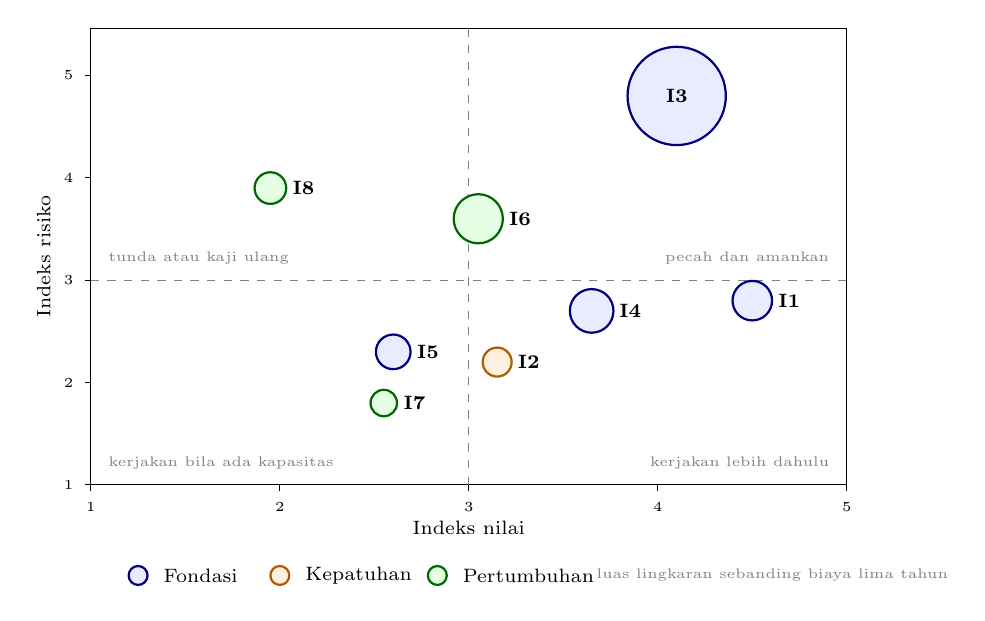
\begin{tikzpicture}[
  font=\scriptsize,
  fondasi/.style={draw=blue!50!black, fill=blue!8, thick},
  kepatuhan/.style={draw=orange!70!black, fill=orange!12, thick},
  tumbuh/.style={draw=green!40!black, fill=green!10, thick},
  kode/.style={font=\scriptsize\bfseries, anchor=west, inner sep=1pt}
]
  % Sumbu: indeks nilai 1 sampai 5 menjadi 0 sampai 9,6 cm,
  % indeks risiko 1 sampai 5 menjadi 0 sampai 5,2 cm.
  \draw (0,0) rectangle (9.6,5.8);
  \draw[gray, dashed] (4.8,0) -- (4.8,5.8);
  \draw[gray, dashed] (0,2.6) -- (9.6,2.6);
  \foreach \nilai/\posisi in {1/0, 2/2.4, 3/4.8, 4/7.2, 5/9.6} {
    \draw (\posisi,0) -- (\posisi,-0.08);
    \node[anchor=north, font=\tiny] at (\posisi,-0.1) {\nilai};
  }
  \foreach \risiko/\posisi in {1/0, 2/1.3, 3/2.6, 4/3.9, 5/5.2} {
    \draw (0,\posisi) -- (-0.08,\posisi);
    \node[anchor=east, font=\tiny] at (-0.1,\posisi) {\risiko};
  }
  \node at (4.8,-0.55) {Indeks nilai};
  \node[rotate=90] at (-0.6,2.9) {Indeks risiko};

  \node[font=\tiny, gray, anchor=south east] at (9.5,0.08) {kerjakan lebih dahulu};
  \node[font=\tiny, gray, anchor=south east] at (9.5,2.68) {pecah dan amankan};
  \node[font=\tiny, gray, anchor=south west] at (0.1,2.68) {tunda atau kaji ulang};
  \node[font=\tiny, gray, anchor=south west] at (0.1,0.08) {kerjakan bila ada kapasitas};

  % Jari-jari 0,09 kali akar biaya, sehingga luas lingkaran sebanding biaya.
  \draw[fondasi] (7.44,4.94) circle (0.624);
  \node[font=\scriptsize\bfseries] at (7.44,4.94) {I3};
  \draw[fondasi] (8.40,2.34) circle (0.251);
  \node[kode] at (8.69,2.34) {I1};
  \draw[fondasi] (6.36,2.21) circle (0.277);
  \node[kode] at (6.67,2.21) {I4};
  \draw[fondasi] (3.84,1.69) circle (0.220);
  \node[kode] at (4.10,1.69) {I5};
  \draw[kepatuhan] (5.16,1.56) circle (0.184);
  \node[kode] at (5.38,1.56) {I2};
  \draw[tumbuh] (4.92,3.38) circle (0.312);
  \node[kode] at (5.27,3.38) {I6};
  \draw[tumbuh] (3.72,1.04) circle (0.168);
  \node[kode] at (3.93,1.04) {I7};
  \draw[tumbuh] (2.28,3.77) circle (0.201);
  \node[kode] at (2.52,3.77) {I8};

  \draw[fondasi] (0.6,-1.15) circle (0.12);
  \node[anchor=west] at (0.8,-1.15) {Fondasi};
  \draw[kepatuhan] (2.4,-1.15) circle (0.12);
  \node[anchor=west] at (2.6,-1.15) {Kepatuhan};
  \draw[tumbuh] (4.4,-1.15) circle (0.12);
  \node[anchor=west] at (4.6,-1.15) {Pertumbuhan};
  \node[anchor=west, font=\tiny, gray] at (6.3,-1.15)
    {luas lingkaran sebanding biaya lima tahun};
\end{tikzpicture}

  \caption{Matriks nilai dan risiko portofolio Medikara, diadaptasi dari
           teknik penilaian nilai bisnis TOGAF dengan tambahan ukuran
           lingkaran untuk biaya}
  \label{fig:ch13-matriks}
\end{figure}

\begin{kasus}[title={Kasus Medikara Health: Memutuskan Portofolio 2026 sampai 2030}]
Misalkan direksi menyediakan pagu Rp60 miliar untuk 2026 sampai 2030,
sedangkan kedelapan inisiatif membutuhkan Rp96 miliar. Bila urutan indeks
nilai diikuti apa adanya, I1 dan I3 menghabiskan Rp55,8 miliar, atau 93
persen pagu. Platform integrasi tidak lagi muat, dan inisiatif kontrol akses
yang menutup temuan audit tidak terdanai. Satu inisiatif berisiko tertinggi
menyerap hampir seluruh anggaran. Pagu ini berlingkup portofolio lima tahun.
Anggaran modernisasi Rp10 miliar pada IT40813 adalah pengandaian latihan
kewenangan keputusan dengan lingkup lebih sempit, termasuk Medikara+ Rp8,4
miliar. Angka itu bukan baris di dalam Rp60 miliar, sehingga keduanya tidak
dijumlahkan.

Tim memakai matriks pada Gambar \ref{fig:ch13-matriks} untuk menyusun usulan
yang berbeda. I1, I2, dan I4 berada di kuadran ``kerjakan lebih dahulu'' dan
didanai penuh. I3 berada di kuadran ``pecah dan amankan'', sehingga hanya
tahap pertamanya yang didanai: pengadaan, konfigurasi, dan percontohan di rumah
sakit Depok senilai Rp22 miliar, dengan titik keputusan K3 pada Maret 2029
sebelum empat rumah sakit lainnya menyusul. I7 murah, berisiko rendah, dan langsung terasa oleh pasien
yang mengeluhkan antrean, sehingga ikut didanai walaupun indeks nilainya
rendah. I6 didanai tahap awalnya saja, Rp6 miliar mulai 2029 untuk mitra
asuransi dan klinik mitra, karena portal mitra bergantung pada platform
integrasi (I4) dan kontrol akses (I2). I5 dan I8 ditunda, karena keduanya
membutuhkan data pasien yang sudah terpadu lewat I1.

Totalnya Rp53 miliar, dan sisanya Rp7 miliar disimpan sebagai cadangan
risiko. Komposisinya 74 persen fondasi (I1, I3 tahap pertama, dan I4), 8
persen kepatuhan (I2), serta 18 persen pertumbuhan (I7 dan I6 tahap awal).

Usulan itu adalah pendanaan awal, bukan pembatalan. Peta jalan Bab 12 tetap memuat
P5, P6, dan P8 sampai selesai. Karena itu sisa I3 Rp26 miliar, I5 Rp6 miliar, dan
sisa I6 Rp6 miliar, seluruhnya Rp38 miliar, diajukan sebagai pendanaan tambahan
pada titik keputusan K2, K3, dan K4 bila kriterianya terpenuhi. Bila tambahan itu
tidak disetujui, paket yang bersangkutan bergeser ke belakang. I8 tetap di luar
peta jalan sampai MPI dan kebijakan AI siap.

Usulan ini dibawa ke komite pengarah TI. Mekanisme keputusan investasi di
tingkat direksi, termasuk siapa yang berhak menyetujui dan bagaimana
keputusannya dipantau, dibahas rinci di mata kuliah IT40813.
\end{kasus}

\section{Menulis Business Case yang Meyakinkan}

\textit{Business case} adalah dokumen keputusan. Dokumen ini meminta satu
keputusan, misalnya ``setujui Rp7,8 miliar untuk 2027 sampai 2031'', dan
memberi alasan yang cukup untuk memutuskannya. Dokumen ini bukan deskripsi
sistem. Panduan HM Treasury menyusun \textit{business case} dari lima sudut
pandang: alasan strategis, nilai ekonomi dari opsi yang dibandingkan,
pengadaan, keuangan, dan pengelolaan pelaksanaannya \cite{c13-hmt2026}. Tabel
\ref{tab:ch13-struktur} menyesuaikan kelima sudut pandang itu dengan artefak
cetak biru yang sudah disusun tim sejak tonggak C1.

\begin{table}[!htb]
  \centering
  \caption{Struktur \textit{business case} dan sumbernya di cetak biru}
  \label{tab:ch13-struktur}
  \footnotesize
  \begin{tabularx}{\textwidth}{>{\raggedright\arraybackslash}p{2.4cm}
                               >{\raggedright\arraybackslash}X
                               >{\raggedright\arraybackslash}X}
    \hline
    \textbf{Bagian} & \textbf{Pertanyaan yang dijawab} &
      \textbf{Sumber di cetak biru} \\
    \hline
    Ringkasan keputusan & Keputusan apa yang diminta, berapa biayanya, dan apa
      hasilnya & Satu halaman, ditulis paling akhir \\
    \hline
    Alasan strategis & Mengapa sekarang, dan strategi mana yang didukung &
      Visi arsitektur C1, \textit{heatmap} kapabilitas Bab 5, \textit{gap
      analysis} Bab 11 \\
    \hline
    Opsi dan nilai & Opsi apa saja yang dibandingkan, termasuk tetap seperti
      sekarang, dan mana yang terbaik & Architecture Decision Record (ADR)
      Bab 10, jaringan manfaat, NPV \\
    \hline
    Pengadaan & Bagaimana membeli atau membangun, dan bentuk kontraknya &
      Keputusan membangun, membeli, atau berlangganan di Bab 9 \\
    \hline
    Keuangan & Berapa biayanya, kapan dikeluarkan, dan dari anggaran mana &
      Tabel TCO, perkiraan biaya \textit{cloud} dari IT40713 \\
    \hline
    Pengelolaan & Siapa memimpin, kapan titik keputusan, dan bagaimana
      manfaat dipantau & Peta jalan Bab 12, pemilik manfaat, tata kelola
      Bab 14 \\
    \hline
    Risiko dan asumsi & Apa yang dapat meleset, dan apa akibatnya pada
      keputusan & Register risiko IT40813, analisis sensitivitas \\
    \hline
  \end{tabularx}
\end{table}

Bahasa untuk direksi berbeda dari bahasa untuk tim proyek. Direksi membaca
ringkasan satu halaman, dan sering hanya itu. Halaman itu memuat lima hal:
keputusan yang diminta, angka utama dalam bentuk rentang, manfaat beserta
pemiliknya, risiko bila inisiatif tidak dijalankan, dan titik keputusan
berikutnya. Istilah teknis diterjemahkan ke akibat bisnisnya. ``MPI''
ditulis sebagai ``satu nomor identitas untuk setiap pasien di 36 fasilitas''.

Analoginya seperti mengusulkan perbaikan jalan kampung di rapat RT. Warga
tidak bertanya tentang jenis aspal. Warga bertanya berapa iurannya, siapa yang
mengerjakan, kapan selesai, apa untungnya bagi rumah masing-masing, dan apa
yang terjadi bila uangnya kurang di tengah jalan. Usulan yang menjawab kelima
pertanyaan itu disetujui lebih cepat daripada usulan yang memuat gambar
teknis paling rapi.

\subsection*{Jujur tentang ketidakpastian}

Pertanyaan kemudian muncul: seberapa besar angka di \textit{business case}
dapat dipercaya? Flyvbjerg dan Budzier menganalisis 1.471 proyek TI dan
menemukan pembengkakan biaya rata-rata 27 persen. Rata-rata itu
menyembunyikan ekor yang berbahaya: satu dari enam proyek membengkak
rata-rata 200 persen, dengan keterlambatan jadwal hampir 70 persen
\cite{flyvbjerg2011}. Angka tunggal tanpa rentang memberi kesan pasti
yang tidak sesuai dengan kenyataan proyek TI.

Dua contoh perbaikan kalimat:

\begin{enumerate}
  \item Kalimat lemah: ``MPI akan meningkatkan efisiensi dan mutu layanan.''
        Kalimat yang lebih kuat: ``MPI menurunkan pemeriksaan lab ulang dari
        18.000 menjadi 6.000 per tahun mulai 2029, senilai Rp1.800 juta per
        tahun, dengan pemilik Direktur Pelayanan. Angka ini bergantung
        pada satu perubahan, yaitu dokter memeriksa riwayat hasil sebelum
        memesan pemeriksaan.''
  \item Kalimat lemah: ``NPV inisiatif ini Rp2.271 juta.'' Kalimat yang lebih
        kuat: ``NPV Rp2.271 juta pada tingkat diskonto 10 persen. Bila
        manfaat tertunda satu tahun, NPV menjadi negatif Rp679 juta. Karena
        itu K2 pada Oktober 2027 memeriksa uji MPI di Depok, dan tinjauan T1
        pada Maret 2028 memeriksa apakah 36 fasilitas sudah memakai MPI.''
\end{enumerate}

Kejujuran itu punya dua konsekuensi. Pertama, \textit{business case} memuat
cadangan risiko dan analisis sensitivitas, bukan hanya skenario terbaik.
Kedua, \textit{business case} terhubung dengan peta jalan Bab 12 lewat titik
keputusan. Setiap titik keputusan adalah kesempatan untuk melanjutkan,
mengubah, atau menghentikan inisiatif berdasarkan manfaat yang sudah
terlihat. Angka biaya juga harus sama dengan perkiraan biaya \textit{cloud} di
IT40713, daftar risiko harus sama dengan register risiko di IT40813, dan
jadwal API mitra harus sama dengan rencana di IT40613. Direksi yang menemukan
dua angka berbeda untuk hal yang sama akan meragukan seluruh dokumen.

% Judul seksi ini terlalu panjang untuk tajuk halaman, sehingga tajuk memakai versi
% pendek, sedangkan daftar isi tetap memakai judul lengkap.
\let\sectionmarkasli\sectionmark
\renewcommand{\sectionmark}[1]{\sectionmarkasli{Aktivitas: Business Case dan Portofolio}}
\section{Aktivitas: Menyusun Business Case dan Memprioritaskan Portofolio}
\let\sectionmark\sectionmarkasli

Aktivitas ini membuat cetak biru tim dapat didanai. Peta jalan dari Bab 12
sudah menjawab urutan pekerjaan. Aktivitas ini menambahkan alasan investasi
untuk inisiatif terpenting dan urutan prioritas untuk seluruh portofolio.
Tim memakai organisasi nyata dengan izin tertulis dan data yang dianonimkan,
atau memakai kasus Medikara Health. Data pribadi pasien dan karyawan tidak
boleh dipakai, termasuk ketika menghitung ukuran seperti jumlah rekam medis
ganda. Yang dipakai hanya angka agregat.

Pembagian peran dalam tim tercantum pada Tabel \ref{tab:ch13-peran}. Peran
digilir seperti pada tonggak sebelumnya.

\begin{table}[!htb]
  \centering
  \caption{Pembagian peran dalam Aktivitas Bab 13}
  \label{tab:ch13-peran}
  \footnotesize
  \begin{tabularx}{\textwidth}{>{\raggedright\arraybackslash}p{2.2cm}
                               >{\raggedright\arraybackslash}X
                               >{\raggedright\arraybackslash}p{3.2cm}}
    \hline
    \textbf{Peran} & \textbf{Tugas} & \textbf{Hasil kerja} \\
    \hline
    Analis bisnis & Memimpin penyusunan \textit{business case}, menurunkan
      manfaat dari tujuan, dan menemui calon pemilik manfaat & Jaringan
      manfaat dan daftar manfaat \\
    \hline
    Analis teknologi & Menyusun perkiraan biaya lisensi, implementasi,
      migrasi, dan operasional beserta sumber tiap angka & Tabel TCO dan arus
      kas \\
    \hline
    Pemodel & Menghubungkan tiap inisiatif dengan kapabilitas dan paket kerja
      di model Archi & Matriks prioritas portofolio \\
    \hline
    Koordinator & Menyelaraskan angka biaya dengan IT40713, risiko dengan
      IT40813, dan jadwal API dengan IT40613 & Daftar asumsi bersama \\
    \hline
  \end{tabularx}
\end{table}

Langkah kerjanya berurutan sebagai berikut.

\begin{enumerate}
  \item Pilih satu atau dua inisiatif prioritas dari paket kerja Bab 11 dan
        peta jalan Bab 12. Pilih inisiatif yang berada di arsitektur transisi
        pertama.
  \item Susun jaringan manfaat dari kanan ke kiri. Tulis tujuan investasi,
        lalu manfaat, perubahan bisnis, perubahan pemungkin, dan teknologi.
        Periksa ulang dari kiri ke kanan, lalu tandai mata rantai yang
        lemah.
  \item Isi daftar manfaat: pemilik, ukuran, nilai awal, target, dan tingkat
        keterukurannya. Konfirmasi tiap pemilik manfaat dengan orangnya
        langsung, bukan hanya ditulis.
  \item Hitung TCO, arus kas, NPV, dan \textit{payback period} memakai
        \berkas{sources/chapter13/data-biaya-manfaat-mpi.csv} sebagai pola.
        Catat sumber setiap angka.
  \item Tulis manfaat yang sulit diukur beserta ukuran penggantinya, dan
        hubungkan pengurangan risikonya dengan register risiko IT40813.
  \item Nilai seluruh inisiatif dengan
        \berkas{sources/chapter13/templat-matriks-prioritas-portofolio.csv}.
        Tetapkan bobot sebelum mengisi skor, gambar matriks nilai dan risiko,
        lalu susun usulan portofolio dalam batas pagu yang diasumsikan.
  \item Tulis \textit{business case} memakai
        \berkas{sources/chapter13/templat-business-case.md}, dimulai dari
        isi, dan ringkasan satu halaman ditulis paling akhir.
\end{enumerate}

Luaran aktivitas ini adalah \textit{business case} untuk satu atau dua
inisiatif prioritas dan portofolio inisiatif berprioritas. Keduanya masuk
tonggak C4 Peta Jalan dan Tata Kelola, bersama peta jalan dari Bab 12, dan
dipresentasikan menjelang UAS (Ujian Akhir Semester). Penilaian singkatnya
memakai empat kriteria:

\begin{itemize}
  \item Setiap manfaat punya pemilik, ukuran, nilai awal, dan target, dan
        tidak ada fitur yang menyamar sebagai manfaat.
  \item Kolom perubahan pada jaringan manfaat terisi dan ikut dianggarkan.
  \item Setiap angka biaya dan manfaat punya sumber, dan angka yang sama di
        IT40713 dan IT40813 tidak berbeda.
  \item Prioritas portofolio dijelaskan dengan bobot yang ditetapkan lebih
        dahulu, dan hal yang dikorbankan ditulis terbuka.
\end{itemize}

\textit{Pendalaman teknis (opsional):} anggota berlatar TI menjalankan
\berkas{sources/chapter13/analisis-business-case.py} untuk inisiatif tim,
lalu menambah satu skenario sensitivitas yang paling relevan bagi
organisasinya, misalnya kenaikan biaya lisensi akibat kurs. Hasilnya
dilampirkan sebagai lampiran \textit{business case}, bukan di ringkasan untuk
direksi.

\section{Ringkasan}

Proyek TI yang selesai tepat waktu dan sesuai anggaran belum tentu berhasil.
Manfaat tidak datang dari teknologi, tetapi dari cara kerja baru yang
dimungkinkan teknologi itu. Manajemen manfaat menjaga agar manfaat itu
dinyatakan sejak awal, diberi pemilik dari sisi bisnis, dan ditinjau setelah
sistem dipakai. Tanpa tahap tinjauan, organisasi tidak pernah tahu apakah
investasinya berhasil.

\textit{Benefits dependency network} menelusuri rantai dari tujuan investasi
sampai teknologi. Jaringan ini disusun dari kanan ke kiri dan diperiksa dari
kiri ke kanan. Kolom yang paling sering dilupakan adalah kedua kolom
perubahan. Pada inisiatif identitas pasien tunggal Medikara, dua dari lima
manfaat bergantung pada satu perubahan sederhana: petugas pendaftaran selalu
mencari di MPI lebih dahulu.

Biaya dihitung sebagai TCO, bukan harga beli. Harga dari penawaran vendor
hanya sekitar 31 persen dari TCO Rp7.800 juta. Dengan manfaat yang dapat
dicairkan sebesar Rp3.400 juta per tahun pada kondisi penuh, inisiatif ini
menghasilkan NPV Rp2.271 juta dan balik modal sekitar 2,3 tahun. Analisis
sensitivitas memperlihatkan bahwa penundaan manfaat satu tahun membuat NPV
negatif, sedangkan kenaikan biaya migrasi 30 persen hanya menguranginya
sedikit.

Manfaat yang sulit diukur tetap ditulis, dengan tingkat keterukuran yang
jujur dan ukuran pengganti yang datanya tersedia. Keselamatan pasien,
kepatuhan, dan pengurangan risiko tidak dipaksa menjadi rupiah yang pasti.
Portofolio dinilai bersama dengan bobot yang ditetapkan lebih dahulu, lalu
dibaca pada matriks nilai dan risiko. Pada kasus Medikara, mengikuti urutan
skor apa adanya justru membuat satu inisiatif berisiko tertinggi menyerap 93
persen pagu.

Pesan utama bab ini: \textit{business case} yang meyakinkan bukan yang
angkanya paling besar, melainkan yang setiap angkanya punya sumber, setiap
manfaatnya punya pemilik, dan setiap ketidakpastiannya ditulis terbuka.
Direksi tidak menuntut kepastian. Direksi menuntut kejujuran tentang apa yang
diketahui, apa yang belum, dan kapan keputusan dapat ditinjau ulang.

\section{Latihan}

\subsection*{Latihan 1: Menulis Ulang Manfaat yang Kabur}

Latihan ini membuktikan bahwa pernyataan seperti ``efisiensi meningkat''
baru dapat dikelola setelah diubah menjadi manfaat yang punya pemilik,
ukuran, nilai awal, dan target.

\begin{enumerate}
  \item Ambil satu pernyataan manfaat yang kabur dari dokumen proyek di
        organisasi tim, atau pakai ``efisiensi pendaftaran meningkat'' dari
        Medikara.
  \item Tanyakan ``efisiensi bagi siapa, diukur dengan apa'', lalu tulis
        perubahan bisnis yang harus terjadi agar manfaat itu muncul.
  \item Tetapkan pemilik manfaat, ukuran beserta sumber datanya, nilai awal,
        target beserta tenggatnya, dan tingkat keterukurannya. Tabel
        \ref{tab:ch13-lat1-contoh} memperlihatkan contoh yang sudah terisi.
  \item Isi Tabel \ref{tab:ch13-lat1-hasil} untuk pernyataan pilihan tim.
  \item Jawab dua pertanyaan berikut. Pertama, apakah manfaat hasil tulisan
        ulang itu dapat dicairkan, dan keputusan tambahan apa yang
        dibutuhkan agar dapat dicairkan? Kedua, bila nilai awalnya belum
        pernah diukur, data apa yang paling murah dikumpulkan sebelum proyek
        dimulai?
\end{enumerate}

\begin{table}[!htb]
  \centering
  \caption{Contoh hasil Latihan 1 yang sudah terisi}
  \label{tab:ch13-lat1-contoh}
  \footnotesize
  \begin{tabularx}{\textwidth}{>{\raggedright\arraybackslash}p{3.2cm}
                               >{\raggedright\arraybackslash}X}
    \hline
    \textbf{Unsur} & \textbf{Isi} \\
    \hline
    Pernyataan awal & Efisiensi pendaftaran meningkat \\
    \hline
    Perubahan bisnis yang dibutuhkan & Petugas mencari pasien di MPI sebelum
      membuat rekam medis baru \\
    \hline
    Manfaat terukur & Median waktu pendaftaran pasien lama turun dari 6
      menjadi 3 menit \\
    \hline
    Pemilik manfaat & Direktur Operasional \\
    \hline
    Ukuran dan sumber data & Selisih waktu buka dan simpan formulir
      pendaftaran, dari catatan SIMRS \\
    \hline
    Nilai awal & 6 menit, median Januari sampai Maret 2026 \\
    \hline
    Target dan tenggat & 3 menit pada Desember 2028 \\
    \hline
    Tingkat keterukuran & Kuantitatif, setara 42.000 jam kerja per tahun,
      tidak dapat dicairkan tanpa keputusan tambahan \\
    \hline
  \end{tabularx}
\end{table}

\begin{table}[!htb]
  \centering
  \caption{Lembar isian Latihan 1}
  \label{tab:ch13-lat1-hasil}
  \footnotesize
  \begin{tabularx}{\textwidth}{>{\raggedright\arraybackslash}p{3.2cm}
                               >{\raggedright\arraybackslash}X}
    \hline
    \textbf{Unsur} & \textbf{Isi} \\
    \hline
    Pernyataan awal & \dots \\
    \hline
    Perubahan bisnis yang dibutuhkan & \dots \\
    \hline
    Manfaat terukur & \dots \\
    \hline
    Pemilik manfaat & \dots \\
    \hline
    Ukuran dan sumber data & \dots \\
    \hline
    Nilai awal & \dots \\
    \hline
    Target dan tenggat & \dots \\
    \hline
    Tingkat keterukuran & \dots \\
    \hline
  \end{tabularx}
\end{table}

\subsection*{Latihan 2: Memilih antara NPV dan Temuan Audit}

Latihan ini membuktikan bahwa NPV yang lebih tinggi tidak otomatis
memenangkan prioritas. Inisiatif A punya NPV lebih tinggi, sedangkan
inisiatif B menutup temuan audit tentang kontrol akses. Pada contoh Medikara,
NPV B tetap negatif walaupun pengurangan kerugian ikut dihitung. Keputusan
mendanai B karena itu bersandar pada temuan audit, kewajiban kepatuhan, dan
dependensi A pada B, bukan pada pengembalian finansial.

\begin{enumerate}
  \item Tetapkan kedua inisiatif. Pada contoh Medikara, A adalah portal
        ekosistem mitra (I6) dan B adalah manajemen identitas dan akses
        terpusat (I2).
  \item Hitung NPV finansial keduanya dengan tingkat diskonto yang sama.
        Pada contoh, A mengeluarkan Rp6.000 juta pada tahun ke-0 lalu Rp1.500
        juta per tahun, dengan manfaat Rp2.000, Rp4.000, Rp5.000, dan Rp6.000
        juta. B mengeluarkan Rp2.200 juta pada tahun ke-0 lalu Rp500 juta per
        tahun, dengan manfaat finansial Rp300 juta per tahun.
  \item Hitung pengurangan nilai harapan kerugian untuk B dari register
        risiko, lalu hitung ulang NPV-nya bila pengurangan itu ikut
        dihitung.
  \item Periksa dependensi: apakah salah satu inisiatif membutuhkan yang
        lain agar aman dijalankan? Bandingkan risiko sisa dengan selera
        risiko organisasi.
  \item Isi Tabel \ref{tab:ch13-lat2-hasil}. Tabel \ref{tab:ch13-lat2-contoh}
        memperlihatkan contoh yang sudah terisi.
  \item Jawab tiga pertanyaan berikut. Pertama, apakah keputusan berubah
        bila pengurangan kerugian B tidak ikut dihitung? Kedua, mengapa
        dependensi A pada B lebih menentukan daripada selisih NPV? Ketiga,
        bagaimana keputusan itu ditulis dalam tiga kalimat untuk direksi?
\end{enumerate}

\begin{table}[!htb]
  \centering
  \caption{Contoh hasil Latihan 2 yang sudah terisi, dalam juta rupiah,
           tingkat diskonto 10 persen (angka fiktif)}
  \label{tab:ch13-lat2-contoh}
  \footnotesize
  \begin{tabularx}{\textwidth}{>{\raggedright\arraybackslash}X
                               >{\raggedright\arraybackslash}p{3.1cm}
                               >{\raggedright\arraybackslash}p{3.1cm}}
    \hline
    \textbf{Aspek} & \textbf{A: portal mitra} & \textbf{B: kontrol akses} \\
    \hline
    TCO lima tahun & 12.000 & 4.200 \\
    \hline
    NPV finansial & 2.223,8 & $-$2.834,0 \\
    \hline
    Pengurangan nilai harapan kerugian & tidak ada & 75 per tahun (R-01 IT40813) \\
    \hline
    NPV bila pengurangan kerugian dihitung & 2.223,8 & $-$2.596,2 \\
    \hline
    Dependensi & Membutuhkan B, karena membuka akses bagi pihak luar & Tidak
      bergantung pada A \\
    \hline
    Posisi terhadap selera risiko & Menambah risiko bila B belum ada &
      Menurunkan risiko ke dalam batas \\
    \hline
    Keputusan & Tahap awal mulai 2029 & Didanai penuh pada 2026 \\
    \hline
  \end{tabularx}
\end{table}

\begin{table}[!htb]
  \centering
  \caption{Lembar isian Latihan 2}
  \label{tab:ch13-lat2-hasil}
  \footnotesize
  \begin{tabularx}{\textwidth}{>{\raggedright\arraybackslash}X
                               >{\raggedright\arraybackslash}p{3.1cm}
                               >{\raggedright\arraybackslash}p{3.1cm}}
    \hline
    \textbf{Aspek} & \textbf{A: \dots} & \textbf{B: \dots} \\
    \hline
    TCO lima tahun & \dots & \dots \\
    \hline
    NPV finansial & \dots & \dots \\
    \hline
    Pengurangan nilai harapan kerugian & \dots & \dots \\
    \hline
    NPV bila pengurangan kerugian dihitung & \dots & \dots \\
    \hline
    Dependensi & \dots & \dots \\
    \hline
    Posisi terhadap selera risiko & \dots & \dots \\
    \hline
    Keputusan & \dots & \dots \\
    \hline
  \end{tabularx}
\end{table}

\subsection*{Latihan 3: Menelusuri Manfaat yang Tidak Tercapai}

Latihan ini membuktikan bahwa manfaat sering hilang walaupun proyeknya
selesai tepat waktu dan sesuai anggaran, dan bahwa titik hilangnya dapat
ditemukan lewat jaringan manfaat.

\begin{enumerate}
  \item Pilih satu proyek yang sudah selesai di organisasi tim. Tim yang
        memakai Medikara memakai skenario pengandaian pada Tabel
        \ref{tab:ch13-lat3-contoh}: misalkan evaluasi tahun pertama aplikasi
        Medikara+ menunjukkan aplikasinya dirilis tepat waktu, tetapi
        manfaatnya jauh di bawah target.
  \item Tulis manfaat yang dijanjikan beserta targetnya, lalu cari angka
        realisasinya.
  \item Susun ulang jaringan manfaat proyek itu dari kanan ke kiri, lalu
        tandai mata rantai yang putus: perubahan bisnis yang tidak terjadi,
        perubahan pemungkin yang tidak dikerjakan, pemilik manfaat yang tidak
        ada, atau manfaat yang tidak dicairkan.
  \item Usulkan satu perbaikan untuk tiap mata rantai yang putus, lalu isi
        Tabel \ref{tab:ch13-lat3-hasil}.
  \item Jawab dua pertanyaan berikut. Pertama, dari seluruh mata rantai yang
        putus, berapa yang berada di kolom teknologi dan berapa di kolom
        perubahan? Kedua, pada tahap mana dari siklus manajemen manfaat
        masalah itu seharusnya sudah terdeteksi?
\end{enumerate}

\begin{table}[!htb]
  \centering
  \caption{Contoh hasil Latihan 3 yang sudah terisi, skenario pengandaian
           Medikara+ (angka fiktif)}
  \label{tab:ch13-lat3-contoh}
  \footnotesize
  \setlength{\tabcolsep}{4pt}
  \begin{tabularx}{\textwidth}{>{\raggedright\arraybackslash}p{2.5cm}
                               >{\raggedright\arraybackslash}p{1.25cm}
                               >{\raggedright\arraybackslash}p{1.35cm}
                               >{\raggedright\arraybackslash}X
                               >{\raggedright\arraybackslash}X}
    \hline
    \textbf{Manfaat dijanjikan} & \textbf{Target} & \textbf{Realisasi} &
      \textbf{Mata rantai yang putus} & \textbf{Perbaikan} \\
    \hline
    Janji temu daring dari total rawat jalan & 40 persen & 12 persen &
      Perubahan bisnis tidak terjadi: dokter tidak membuka jadwal di aplikasi
      & Kuota jadwal daring ditetapkan, Direktur Operasional menjadi
      pemilik \\
    \hline
    Antrean pendaftaran pagi turun & 30 persen & 5 persen & Perubahan bisnis
      tidak terjadi: pasien daring tetap mendaftar ulang di loket & Jalur
      lapor hadir khusus pasien daring \\
    \hline
    Biaya pusat panggilan turun & Rp600 juta & Rp0 & Manfaat tidak dicairkan:
      staf pusat panggilan tidak dialihkan & Rencana pengalihan staf
      bertahap \\
    \hline
  \end{tabularx}
\end{table}

\begin{table}[!htb]
  \centering
  \caption{Lembar isian Latihan 3}
  \label{tab:ch13-lat3-hasil}
  \footnotesize
  \setlength{\tabcolsep}{4pt}
  \begin{tabularx}{\textwidth}{>{\raggedright\arraybackslash}p{2.5cm}
                               >{\raggedright\arraybackslash}p{1.25cm}
                               >{\raggedright\arraybackslash}p{1.35cm}
                               >{\raggedright\arraybackslash}X
                               >{\raggedright\arraybackslash}X}
    \hline
    \textbf{Manfaat dijanjikan} & \textbf{Target} & \textbf{Realisasi} &
      \textbf{Mata rantai yang putus} & \textbf{Perbaikan} \\
    \hline
    \dots & \dots & \dots & \dots & \dots \\
    \hline
    \dots & \dots & \dots & \dots & \dots \\
    \hline
    \dots & \dots & \dots & \dots & \dots \\
    \hline
  \end{tabularx}
\end{table}
